\subsection{Свойства интеграла, выраженные неравенствами. Неравенство Коши — Буняковского}

В данном билете рассматриваются свойства определенного интеграла Римана, которые позволяют оценивать его значение через значения самой функции. Лектор подчеркивает, что эти теоремы часто являются «спасательным кругом» на экзамене.

\subsubsection*{1. Интегрирование неравенств и оценка модуля}

\begin{theorem}[Об оценке модуля интеграла]
Если функция $f(x)$ интегрируема на отрезке с концами $a$ и $b$, то выполняется неравенство:
\[ \left| \int\limits_a^b f(x) dx \right| \le \left| \int\limits_a^b |f(x)| dx \right| \]
В частности, если $a < b$, то:
\[ \left| \int\limits_a^b f(x) dx \right| \le \int\limits_a^b |f(x)| dx \]
\end{theorem}

\begin{tcolorbox}[title=Доказательство, breakable]
Рассмотрим случай $a < b$. Составим интегральную сумму Римана для функции $f(x)$:
\[ \sigma(f, P, \xi) = \sum_{j=1}^n f(\xi_j) \Delta x_j \]
По свойству модуля суммы (неравенство треугольника):
\[ |\sigma(f, P, \xi)| = \left| \sum_{j=1}^n f(\xi_j) \Delta x_j \right| \le \sum_{j=1}^n |f(\xi_j)| \cdot |\Delta x_j| \]
Так как $a < b$, то $\Delta x_j > 0$, и правая часть есть интегральная сумма для функции $|f(x)|$:
\[ |\sigma(f, P, \xi)| \le \sigma(|f|, P, \xi) \]
Переходя к пределу при $\lambda(P) \to 0$ и учитывая, что интегрируемость $f$ влечет интегрируемость $|f|$, получаем:
\[ \left| \int\limits_a^b f(x) dx \right| \le \int\limits_a^b |f(x)| dx \]
Случай $a > b$ доказывается переменой пределов интегрирования, что порождает знак минус, поглощаемый внешним модулем.
\end{tcolorbox}

\begin{theorem}[Сравнение интегралов]
Пусть $a \le b$ и функции $f(x), g(x)$ интегрируемы на $[a, b]$. Если для всех $x \in [a, b]$ выполняется $f(x) \le g(x)$, то:
\[ \int\limits_a^b f(x) dx \le \int\limits_a^b g(x) dx \]
\end{theorem}

\begin{tcolorbox}[title=Доказательство, breakable]
Для любого разбиения $P$ и набора отмеченных точек $\xi$ из условия $f(\xi_j) \le g(\xi_j)$ и $\Delta x_j \ge 0$ следует:
\[ \sum_{j=1}^n f(\xi_j) \Delta x_j \le \sum_{j=1}^n g(\xi_j) \Delta x_j \implies \sigma(f, P, \xi) \le \sigma(g, P, \xi) \]
Переходя к пределу при $\lambda(P) \to 0$, в силу сохранения знака неравенства при предельном переходе, получаем искомое утверждение.
\end{tcolorbox}

\begin{consequence}[Оценка интеграла через грани]
Если $a \le b$ и на отрезке $[a, b]$ справедливо $m \le f(x) \le M$, то:
\[ m(b-a) \le \int\limits_a^b f(x) dx \le M(b-a) \]
\end{consequence}

\subsubsection*{2. Неравенство Коши — Буняковского}

Это фундаментальное неравенство связывает интеграл от произведения двух функций с интегралами от их квадратов. Лектор отмечает его аналогию со скалярным произведением векторов.

\begin{theorem}[Неравенство Коши — Буняковского]
Пусть функции $f(x)$ и $g(x)$ интегрируемы на отрезке $[a, b]$. Тогда выполняется неравенство:
\[ \left( \int\limits_a^b f(x) g(x) dx \right)^2 \le \int\limits_a^b f^2(x) dx \cdot \int\limits_a^b g^2(x) dx \]
\end{theorem}

\begin{tcolorbox}[title=Доказательство, breakable]
1. Заметим, что если функции $f$ и $g$ интегрируемы, то функции $f^2$, $g^2$ и их произведение $fg$ также интегрируемы на $[a, b]$.

2. Рассмотрим произвольное действительное число $\lambda \in \R$ и составим вспомогательную функцию:
\[ h(x) = (\lambda f(x) + g(x))^2 \ge 0 \]
В силу линейности интеграла и того, что интеграл от неотрицательной функции на $[a, b]$ ($a \le b$) неотрицателен:
\[ I(\lambda) = \int\limits_a^b (\lambda f(x) + g(x))^2 dx \ge 0 \]

3. Раскроем квадрат под интегралом:
\[ \int\limits_a^b \left( \lambda^2 f^2(x) + 2\lambda f(x)g(x) + g^2(x) \right) dx \ge 0 \]
\[ \lambda^2 \left( \int\limits_a^b f^2(x) dx \right) + 2\lambda \left( \int\limits_a^b f(x)g(x) dx \right) + \left( \int\limits_a^b g^2(x) dx \right) \ge 0 \]

4. Полученное выражение является квадратным трехчленом относительно $\lambda$ вида $A\lambda^2 + 2B\lambda + C \ge 0$, где:
\[ A = \int\limits_a^b f^2(x) dx, \quad B = \int\limits_a^b f(x)g(x) dx, \quad C = \int\limits_a^b g^2(x) dx \]

5. Чтобы квадратичная форма была всегда неотрицательной, необходимо и достаточно, чтобы её дискриминант (точнее, $D/4$) был неположителен:
\[ \frac{D}{4} = B^2 - AC \le 0 \implies B^2 \le AC \]
Подставляя значения $A, B$ и $C$, получаем:
\[ \left( \int\limits_a^b f(x) g(x) dx \right)^2 \le \int\limits_a^b f^2(x) dx \cdot \int\limits_a^b g^2(x) dx \]
Теорема доказана.
\end{tcolorbox}

\subsubsection*{3. Геометрический и физический смысл}
Неравенства с интегралами отражают естественные свойства площадей и физических величин:
\begin{itemize}
    \item Сравнение: если один график лежит выше другого, то и площадь под ним больше.
    \item Оценка модуля: площадь «суммарного отклонения» всегда не меньше модуля «чистого перемещения» (где части ниже оси вычитаются).
    \item Коши — Буняковский: в пространстве функций это неравенство означает, что «косинус угла» между функциями-векторами не превосходит единицы по модулю.
\end{itemize}

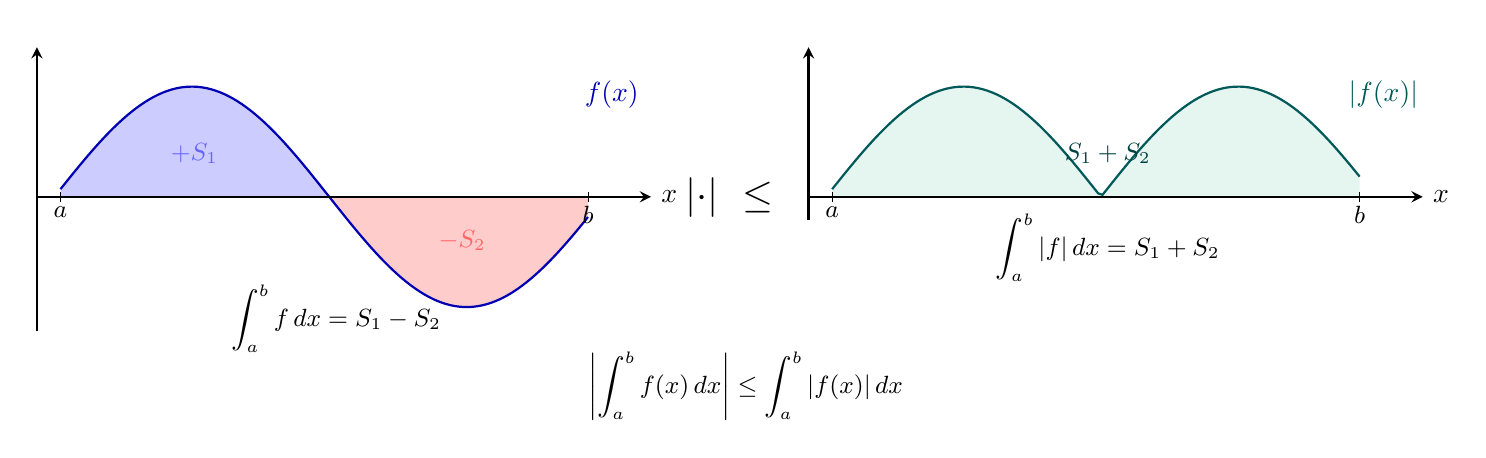
\begin{tikzpicture}[>=stealth,scale=1.0]
 
\pgfmathdeclarefunction{ff}{1}{%
  \pgfmathparse{1.4*sin(deg(\x*0.9-0.2))}%
}
\pgfmathdeclarefunction{fabs}{1}{%
  \pgfmathparse{abs(1.4*sin(deg(\x*0.9-0.2)))}%
}
 
\def\xa{0.3}
\def\xb{7.0}
 
%=== Левая картинка: f(x) со знаком ===
\begin{scope}
 
  % Область f>0 (синяя)
  \fill[blue!20,domain=\xa:3.73,samples=60]
    plot(\x,{ff(\x)}) -- (3.73,0) -- (\xa,0) -- cycle;
  % Область f<0 (красная)
  \fill[red!20,domain=3.73:\xb,samples=60]
    plot(\x,{ff(\x)}) -- (\xb,0) -- (3.73,0) -- cycle;
 
  \draw[blue!70!black,thick,domain=\xa:\xb,samples=120]
    plot(\x,{ff(\x)});
 
  % Ось x, y
  \draw[->,thick] (0,0)--(7.8,0) node[right]{$x$};
  \draw[->,thick] (0,-1.7)--(0,1.9) node[above]{};
 
  % Метки a, b
  \draw (\xa,0.06)--(\xa,-0.06); \node[below,font=\small] at (\xa,0){$a$};
  \draw (\xb,0.06)--(\xb,-0.06); \node[below,font=\small] at (\xb,0){$b$};
 
  % Метки площадей
  \node[blue!60,font=\small] at (2.0,0.55){$+S_1$};
  \node[red!60,font=\small] at (5.4,-0.55){$-S_2$};
 
  % Подпись интеграла
  \node[font=\small] at (3.8,-1.55)
    {$\displaystyle\int_a^b f\,dx = S_1 - S_2$};
 
  \node[blue!70!black,font=\itshape] at (7.3,1.3){$f(x)$};
\end{scope}
 
% знак ≤ по центру
\node[font=\Large] at (8.8,0) {$\Bigl|\cdot\Bigr|\ \leq$};
 
%=== Правая картинка: |f(x)| ===
\begin{scope}[xshift=9.8cm]
 
  \fill[green!20!teal!10,domain=\xa:\xb,samples=120]
    plot(\x,{fabs(\x)}) -- (\xb,0) -- (\xa,0) -- cycle;
 
  \draw[teal!70!black,thick,domain=\xa:\xb,samples=120]
    plot(\x,{fabs(\x)});
 
  \draw[->,thick] (0,0)--(7.8,0) node[right]{$x$};
  \draw[->,thick] (0,-0.3)--(0,1.9) node[above]{};
 
  \draw (\xa,0.06)--(\xa,-0.06); \node[below,font=\small] at (\xa,0){$a$};
  \draw (\xb,0.06)--(\xb,-0.06); \node[below,font=\small] at (\xb,0){$b$};
 
  \node[teal!50!black,font=\small] at (3.8,0.55){$S_1+S_2$};
 
  \node[font=\small] at (3.8,-0.65)
    {$\displaystyle\int_a^b|f|\,dx = S_1 + S_2$};
 
  \node[teal!70!black,font=\itshape] at (7.3,1.3){$|f(x)|$};
\end{scope}
 
%--- Общая подпись ---
\node[font=\small] at (9.0,-2.4)
  {$\displaystyle\left|\int_a^b f(x)\,dx\right|\le\int_a^b|f(x)|\,dx$};
 
\end{tikzpicture}